\begin{frame}
\frametitle{Folds}
\framesubtitle{folding left and right}

\begin{itemize}
\item We are going to be discussing the \lstinline[basicstyle=\ttfamily]$foldl$ and \lstinline[basicstyle=\ttfamily]$foldr$ functions on \textbf{cons lists}.
\item In the Scala programming language, these are called \lstinline[basicstyle=\ttfamily]$foldLeft$ and \lstinline[basicstyle=\ttfamily]$foldRight$.
\item The C\# programming language provides an approximation for \lstinline[basicstyle=\ttfamily]$foldl$ called \lstinline[basicstyle=\ttfamily]$Aggregate$ (there is no \lstinline[basicstyle=\ttfamily]$foldr$ equivalent).
\item Our discussion is language-independent and so applies equally to Haskell, Scala and more. 
\end{itemize}

\end{frame}


\begin{frame}
\frametitle{Folds}
\framesubtitle{explanations}

\center
There are all types of explanations of list fold functions out there.

\end{frame}


\begin{frame}
\frametitle{Folds}
\framesubtitle{diagrams}

\begin{block}{Fold Diagrams}

\begin{figure}
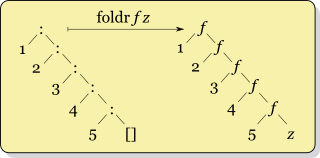
\includegraphics[width=0.5\textwidth,natwidth=320,natheight=158]{res/image/Right-fold-transformation.png}
\end{figure}

\end{block}

\end{frame}


\begin{frame}
\frametitle{Folds}
\framesubtitle{descriptions}

\begin{block}{Short, concise descriptions}

\begin{itemize}
\item \lstinline[basicstyle=\ttfamily]$foldl$ applies a function to a list, associating to the left.
\begin{itemize}
  \item \lstinline[basicstyle=\ttfamily]$\\f z -> (f (f (f a z) b) c)$
\end{itemize}
\item \lstinline[basicstyle=\ttfamily]$foldr$ applies a function to a list, associating to the right. 
\begin{itemize}
  \item \lstinline[basicstyle=\ttfamily]$\\f z -> (f a (f b (f c z)))$
\end{itemize}
\end{itemize}

\end{block}

\end{frame}


\begin{frame}
\frametitle{Folds}
\framesubtitle{questions}

\begin{block}{But then I am hit with more questions}

\begin{itemize}
\item How does folding right start from the right but work on infinite lists?
\item How do I recognise when it is appropriate to use a fold function?
\item When do I choose to use one over the other?
\end{itemize}

\end{block}

\end{frame}
